\documentclass[12pt]{article}
\usepackage{graphicx} %Required for diagrams
\usepackage{bookmark}
\usepackage{hyperref}

\begin{document}

\begin{titlepage}
	\begin{center}
		
		\begin{figure}[t]
			\centering
			
\includegraphics[width=350px]{UP_Logo.png}
		\end{figure}
		
		% Title
		\textsc{\LARGE COS301 Mini Project Functional \newline\newline Requirements Specification}
		
		%\begin{minipage}{0.4\textwidth}
		\textbf{\newline Group 2a} \\
		\begin{flushright} \large
			Matthew Gouws \emph{u11008602} \newline
			Neo Thobejane \emph{u11215918} \newline
			Roger Tavares \emph{u10167324} \newline
			Rendani Dau \emph{u13381467} \newline
			Ivan Henning \emph{u13008219} \newline
			Name Surname \emph{uxxxxxxxx} \newline
			Name Surname \emph{uxxxxxxxx} \newline
			Name Surname \emph{uxxxxxxxx} \newline
		\end{flushright}
		%\end{minipage}
		
		\vfill
		
		{\large Version }
		\\
		{\large \today}
		
	\end{center}
\end{titlepage}


\section{History}
\begin{tabular}{|l|l|l|}

\hline
Date & Version & Description\\ %NOTE: Necessary for [updated by] ?
\hline
17-02-2015 & Version 0.1 & Document Template Created\\ %February 17 - Matthew (Took the date that the document was on github)
17-02-2015 & Version 0.1.1 & Auto title page added \\% %February 17 - Szymon (Took the date that the document was on github)
17-02-2015 & Version 0.2 & UP Logo Added \\%February 17 - Roger (Date Taken from github)
18-02-2015 & Version 0.2.1 & Intro, Purpose, Conventions and Description Added\\%February 18 - Matthew (Date Taken from GitHub
19-02-2015 & Version 0.2.2 & Added Skeleton for Required functionality \\%February 19 - Matthew (Date Taken from GitHub
19-02-2015 & Version 0.2.3 & Added Bulk of Points - Roger \\%February 19 - Roger (Date Taken from github)
20-02-2015 & version 0.2.4 & Added point Headings - David \\%February 20 - David (Date Taken from github)
20-02-2015 & version 0.2.5 & Added Use Cases - Matthew \\%February 20 - Matthew (Date Taken from github)
20-02-2015 & version 0.2.6 & Added Use Cases - Roger \\%February 20 - Roger (Date Taken from github)
22-02-2015 & version 0.2.7 & Added Details on points - David \\%February 22 - David (Date Taken from github)
23-02-2015 & Version 0.3 & Updated Use Case prioritization and fixed newPage \\ & & with Clearpage \\%February 23 - Matthew (Date Taken from GitHub
23-02-2015 & version 0.3.1 & Added points - Rendani \\%February 23 - Rendani (Date Taken from github)
23-02-2015 & version 0.3.2 & Added points - Neo \\%February 23 - Neo (Date Taken from github)
23-02-2015 & version 0.3.3 & Added Points - Ivan \\%February 23 - Ivan (Date Taken from github)
24-02-2015 & version 0.3.4 & Added Diagrams - Ivan \\%February 24 - Ivan (Date Taken from github)
24-02-2015 & version 0.3.5 & Changed Original Layout removed unnecessary sections \\%February 24 - Matthew (Date Taken from github)
24-02-2015 & version 0.3.6 & Added Diagrams - David \\%February 24 - David (Date Taken from github)
24-02-2015 & version 0.3.7 & Added Diagrams - Roger \\%February 24 - Roger (Date Taken from github)
24-02-2015 & version 0.4 & Added Project Scope\\%February 24 - Roger (Date Taken from github)
24-02-2015 & version 0.4.1 & Added Diagrams - Szymon \\%February 24 - Szymon (Date Taken from github)
25-02-2015 & version 0.4.2 & Added points - Keagan \\%February 25 - Keagan (Date Taken from github)
25-02-2015 & version 0.4.3 & Added Diagrams - Neo \\%February 25 - Neo (Date Taken from github)
25-02-2015 & version 0.4.4 & Added points - Ivan \\%February 25 - Ivan (Date Taken from github)
25-02-2015 & version 0.4.5 & Fixed Clearpage Newpage problems \\%February 25 - Matthew (Date Taken from github)
25-02-2015 & version 0.4.6 & Added Domain Model - David \\%February 25 - David (Date Taken from github)
25-02-2015 & version 0.4.7 & Added Domain Model - Syzmon \\%February 25 - Syzmon (Date Taken from github)
26-02-2015 & version 0.5 & Added Combined, Master, Use case \\%February 26 - Keagan (Date Taken from github)
26-02-2015 & version 0.5.1 & Added Diagrams - Neo \\%February 26 - Neo (Date Taken from github)



\end{tabular}

\newpage
\tableofcontents
\newpage
\listoffigures
\newpage

\section{Introduction}
The Computer Science Education Didactic and Application Research (CSEDAR) from the university of Pretoria. Have approached us in building a software platform to create a collaborative community by means of an online discussion. To aid students to excel in problem solving as  group. Such a tool already exists for students to use however this tool lacks certain functionality, Lecturer - Student interaction, often students are unaware of who is higher ranked in terms of the course (Teaching Assistant, Tutor, Lecturer \& student).

\subsection{Purpose}
This document serves to present the clients requirements on a functional level by use of use-case diagrams, Domain models, pre- \& post conditions as well as possible input-output pairs.

\subsection{Document Conventions}
A ranking system of importance is used for the functional requirements based on a 'star' system with 
\\****** - Critical
\\*****  - Important
\\ ****  - Somewhat important
\\  ***  - Nice to have
\\  **   - Not considered


\subsection{Project Scope}
The scope of this project is to create a Buzz Space system to integrate into the Computer Science Department's website at the University of Pretoria. This software solution will provide an online forum that is both organized and interactive to engage the students in their studies. The project can then later also be expanded to multiple universities and institutions.

\subsection{References}
Tutorial on Use case diagrams - \url{http://www.tutorialspoint.com/uml/uml_use_case_diagram.htm}

\section{System Description}
Buzz will be a complete software unit which is to be integrated seamlessly with existing web servers to be used by courses to encourage the use of online discussion. Users will be able to climb ranks up the online discussion forum and achieve more functionality as they progress. The system will also have certain functionality incorporated into awarding users marks if required so by the teaching staff. Teaching staff will also be able to archive and summarise threads. Users will also only be able to post in threads which pertain to them at that specific time, thus having a thread become 'Ancient' and hence archived no new information may be added to said thread.
\newpage %Use case diagram on its own page...quite large (Entire Combined Use Case)

\section{Functional Requirements}

\subsection{Use Cases}
\begin{figure}[h]
	\centering
	\includegraphics[height=600px]{"Diagrams/Use Case/CombinedUseCase".jpg}
	\caption{Combined Use Case of Entire System}
\end{figure}
\clearpage

\subsubsection{Use Case Prioritization}
\textbf{Critical:}
\begin{itemize}
\item Users must be able to create, Read, update and delete posts.
\item Users must only be able to post on specific threads/levels based on their level.
\item Staff should be able to summarize, close/hide threads and move posts around.
\item Buzz must integrate seamlessly with any host site.
\end{itemize}
\textbf{Important:}
\begin{itemize}
\item The system should keep track of what posts have been read by a specific user and highlight unread posts.
\item The system should allow for social tagging, allowing users to easily locate threads on what they are looking for.
\end{itemize}
\textbf{Important-Nice to have:} 
\begin{itemize}
\item The post length should be restricted. Users of higher levels can post and embed Pictures, Videos etc.
\item A users status should automatically update based on their participation.
\item Post should be able to be up-voted, shown higher in the thread.
\item Statistics should be available for each student displaying their marks, and visual reporting of their level.
\end{itemize}
\newpage
\textbf{Nice to have:}
\begin{itemize}
\item Semi-automated thread summary creation.
\item Create an automated template based on Message and other users.
\item Provide searching and filtering.
\item Enhancement of posts, such as Rich-text-format editor.
\item Apply organization of content based on tags, base structure or ownership structure.
\item Detect if a post is plagiarised.
\item Detect if Netiquette rule are broken.
\end{itemize}

\newpage %Use case diagram on its own page...quite large (Entire Combined Use Case)
\subsection{Required Functionality}
The Following system processes detail the functional requirements of the individual points.
\begin{enumerate}
  \item Users must create, Update and delete posts. % Point 1 - Syzmon
  	\begin{enumerate}
  		\item Create Post
  		\begin{enumerate}
    		\item Elaboration - In order for the user to communicate with others in the Buzz space, (s)he need to be able to 				create posts. User must have sufficient permissions to post in certain areas of the Buzz space. This function is not available to guests.
   	 		\item Importance - *****, Critical
   	 		\item Dependency level - With out the ability to create posts users will not be able to communicate with one another, which makes the Buzz space useless.
   	 		\item Pre-conditions
   			\begin{enumerate}
    			\item User must have necessary permissions.
    			\item Buzz space must exist.
    			\item User must be registered.
    			\item User must be logged in and not a guest.
    		\end{enumerate}
     		\item Post-conditions
    		\begin{enumerate}
  	  			\item Post will be successfully created.
   	 		\end{enumerate}
   	 		\item Requester - Client
  		\end{enumerate}
  	\begin{figure}[h]
  		\centering
  		\includegraphics[width=300px]{"Diagrams/Use Case/Use_Case_Diagram_Create_Post".png}
  		\caption{Create post use case}
  	\end{figure}
  	\begin{figure}[h]
  		\centering
  		\includegraphics[width=300px]{"Diagrams/Process Specification/Activity_Diagram_Create_Post_AD".png}
  		\caption{Create post activity diagram}
  	\end{figure}
  	\clearpage
  	\newpage
  		\item Read Post
  		\begin{enumerate}
  			\item Elaboration - This function allows users read posts made by other users of the Buzz space.
   	 		\item Importance - *****, Critical
   	 		\item Dependency level - This function is very important because without it, the Buzz space is useless as users will not be able to read each others posts, which defeats the purpose of the Buzz space.
   	 		\item Pre-conditions
   			\begin{enumerate}
    			\item Buzz space and post must exist.
    			\item Access to Buzz space.
    		\end{enumerate}
     		\item Post-conditions
    		\begin{enumerate}
  	  			\item If the user is not a guest post will be marked as read.
   	 		\end{enumerate}
   	 		\item Requester - Client
  		\end{enumerate}
  	\begin{figure}[h]
  		\centering
  		\includegraphics[width=300px]{"Diagrams/Use Case/Use_Case_Diagram_Read_Post".png}
  		\caption{Read post use case}
  	\end{figure}
  	\begin{figure}[h]
  		\centering
  		\includegraphics[width=300px]{"Diagrams/Process Specification/Activity_Diagram_Read_Post_AD".png}
  		\caption{Read post activity diagram}
  	\end{figure}
  	\newpage
  	\clearpage
  		\item Update Post
  		\begin{enumerate}
  			\item Elaboration - This function allows the user to update his/her post. It is only available to certain users such as the owner of the post or the moderators.
   	 		\item Importance - *****, Critical
   	 		\item Dependency level - Updating posts is another important process needed in the Buzz space. People often make mistakes in their posts and have to correct it. The ability to update the post will help achieve that.
   	 		\item Pre-conditions
   			\begin{enumerate}
    			\item User must be either the owner of the post or the moderator of that Buzz space.
    		\end{enumerate}
     		\item Post-conditions
    		\begin{enumerate}
  	  			\item Post will be updated.
   	 		\end{enumerate}
   	 		\item Requester - Client
  		\end{enumerate}
  	\begin{figure}[h]
  		\centering
  		\includegraphics[width=300px]{"Diagrams/Use Case/Use_Case_Diagram_Update_Post".png}
  		\caption{Update post use case}
  	\end{figure}
  	\begin{figure}[h]
  		\centering
  		\includegraphics[width=300px]{"Diagrams/Process Specification/Activity_Diagram_Update_Post_AD".png}
  		\caption{Update post activity diagram}
  	\end{figure}
  	\clearpage
  	\newpage
  		\item Delete Post
  		\begin{enumerate}
  			\item Elaboration - Deleting posts allows for users to remove their post from a Buzz space and also allows the moderators to delete posts that they think are not suitable for the Buzz space.
   	 		\item Importance - *****, Critical
   	 		\item Dependency level - The deleting of a post is also very important to a Buzz space. Owners of a post would like to remove their post if they think it is not relevant to the topic and moderators should be able to delete user posts if they think the post is not relevant.
   	 		\item Pre-conditions
   			\begin{enumerate}
    			\item User must be either the owner of the post or the moderator of that Buzz space.
    			\item Post must exist.
    		\end{enumerate}
     		\item Post-conditions
    		\begin{enumerate}
  	  			\item Post will be marked as deleted and hidden from Buzz space. Post is not physically deleted from database.
   	 		\end{enumerate}
   	 		\item Requester - Client
  		\end{enumerate}
  	\begin{figure}[h]
  		\centering
  		\includegraphics[width=300px]{"Diagrams/Use Case/Use_Case_Diagram_Delete_Post".png}
  		\caption{Delete post use case}
  	\end{figure}
  	\begin{figure}[h]
  		\centering
  		\includegraphics[width=300px]{"Diagrams/Process Specification/Activity_Diagram_Delete_Post_AD".png}
  		\caption{Delete post activity diagram}
  	\end{figure}
  	\begin{figure}[h]
  		\centering
  		\includegraphics[width=300px]{"Diagrams/UML/Class_Diagram_CRUD".png}
  		\caption{Create, read, update and delete posts class diagram}
  	\end{figure}
  	\clearpage
  	\end{enumerate}
%Diagram to go here \includegraphics[width=350px]{UseCases/File_Name.png}
\clearpage %Each point on a new page
  \item Keep track of who has read what and highlight unread messages for each user. % Point 2 - Rendani
  \begin{enumerate}
    \item Elaboration - This process will allow the student/user to see which thread he/she still has to read by applying some form of emphasis on the thread. It will also allow a lecturer/board moderator to view read statistics of a thread such as how many students have read a thread and who those students are.
    \item Importance - ****
    \item Dependency level - Highlighting unread posts is important because it will allow users to efficiently follow discussions without having to find specific points where they last read and this in turn will help users post replies faster keeping discussions relevant. It is also important that the lecturer/moderator can view statistics of who has read which posts as this will give them an idea of how many students follow discussions and who those students are.
    \item Pre-conditions
    \begin{enumerate}
    	\item A user must be logged in and registered for that particular buzz space.
    	\item A user must be logged in and have elevated privileges, such as lecturer/moderator status, to view read statistics of a post
    \end{enumerate}
        \item Post-conditions
    \begin{enumerate}
    	\item User is presented with formatted view highlighting unread threads
    	\item User(lecturer) is presented with read statistics of a particular thread
    \end{enumerate}
    \item Requester - Client
  \end{enumerate}
  \begin{figure}[h]
  		\centering
  		\includegraphics[width=300px]{"Diagrams/Use Case/readStatisticsUseCase".png}
  		\caption{Highlighting/Read Statistics Use Case}
  	\end{figure}
  	\begin{figure}[h]
  		\centering
  		\includegraphics[width=300px]{"Diagrams/Process Specification/ReadStatisticsActivity".png}
  		\caption{Highlighting/Read Statistics Activity}
  	\end{figure}
	%\includegraphics[width=350px]{"Diagrams/Use Case/Dau use case 1".png}
\clearpage %Each point on a new page
  \item Restrict the length of messages and the type of content allowed in messages based
on the level where it is posted as well as on the status of the user posting the
message.  % Point 3 - David
  \begin{enumerate}
    \item Elaboration - Restrictions on the length of message should be configurable by policy, according to user level and post location. This will allow Buzz Space creators specific control over content type and post length for users of different level/rank.
    \item Importance - ***
    \item Dependency level - Relies on the ranking system to be implemented and provide a user's level/rank. Two policies must be set by the Buzz Space creator, one for message length according to level/rank, and one for permitted content types according to level/rank.
    \item Pre-conditions
    \begin{enumerate}
    	\item User must belong to a Buzz Space.
    	\item User must attempt to post.
	\item Policies must be acquired.
    \end{enumerate}
        \item Post-conditions
    \begin{enumerate}
    	\item User successfully posted a post that contains only permitted content types.
    	\item User successfully posted a post that contains less than or equal to the permitted character length.
    \end{enumerate}
    \item Requester - System
  \end{enumerate}
\begin{figure}[h]
  	\centering
  	\includegraphics[width=400px]{"Diagrams/Use Case/UseCasePoint03".png}
  	\caption{Message Length and Content Restriction Use Case}
  \end{figure}
  \begin{figure}[h]
  		\centering
  		\includegraphics[width=300px]{"Diagrams/Process Specification/ProcessSpecPoint03".png}
  		\caption{Message Length and Content Restriction activity diagram}
  	\end{figure}
	\begin{figure}[h]
  		\centering
  		\includegraphics[width=300px]{"Diagrams/UML/UML_Point03".png}
  		\caption{Message Length and Content Restriction activity diagram}
  	\end{figure}
%Diagram to go here \includegraphics[width=350px]{UseCases/File_Name.png}
\clearpage %Each point on a new page
   \item Restrict users to post on specified levels based on their status. % Point 4 - Roger
  \begin{enumerate}
    \item Elaboration - User interaction with the current Buzz space must be configurable by policy to allow users with higher levels to post to the Buzz space on higher levels such as directly below the main post while restricting low level users to only post in lower levels like sub level posts or even sub sub level posts. This allows high level users to post higher up in the Buzz spaces hierarchy while restricting low level users to the bottom. 
    \item Importance - ****
    \item Dependency level - Relies on the ranking system to be implemented so that it can request user levels. A policy to govern the levels has to be supplied by the creator of the Buzz space.
    \item Pre-conditions
    \begin{enumerate}
    	\item User must be part of the specific Buzz space.
    	\item Policy acquired.
    	\item User must try to post.
    \end{enumerate}
        \item Post-conditions
    \begin{enumerate}
    	\item User successfully posted to the correct level as specified in the policy.
    \end{enumerate}
    \item Requester - System (This is an automated system requirement)
  \end{enumerate}
\begin{figure}[h]
	\centering
	\includegraphics[width=345px]{"Diagrams/Use Case/UserRestrictionByLevel UseCase".png}
	\caption{User Post Restriction By User Level Use Case}
\end{figure}
\begin{figure}[h]
	\centering
	\includegraphics[width=400px]{"Diagrams/Process Specification/UserRestrictionByLevel Process Spec".png}
	\caption{User Post Restriction By User Level Process Specification}
\end{figure}
\begin{figure}[h]
	\centering
	\includegraphics[width=400px]{"Diagrams/UML/UserRestrictionByLevel UML".png}
	\caption{User Post Restriction By User Level UML}
\end{figure}
%Diagram to go here \includegraphics[width=350px]{UseCases/File_Name.png}
\clearpage %Each point on a new page
   \item  Allow staff to manage content i.e. summarise, close or hide threads and move things around.% Point 5 - Ivan
  \begin{enumerate}
    \item Elaboration - After a staff member has viewed through the thread he can choose to add a summary of what the thread is about. He can then close the thread to stop further posts but still visible to other members or hide the thread to make it only visible to selected members.
    \item Importance - ****.
    \item Dependency level - Relies on the user having the rights or high enough rank/owner of the thread.
    \item Pre-conditions
    \begin{enumerate}
    	\item The user has a high enough rank.
    	\item The user is the owner of the thread.
    \end{enumerate}
        \item Post-conditions
    \begin{enumerate}
    	\item N/A.
    	\item N/A.
    \end{enumerate}
    \item Requester
  \end{enumerate}
%Diagram to go here 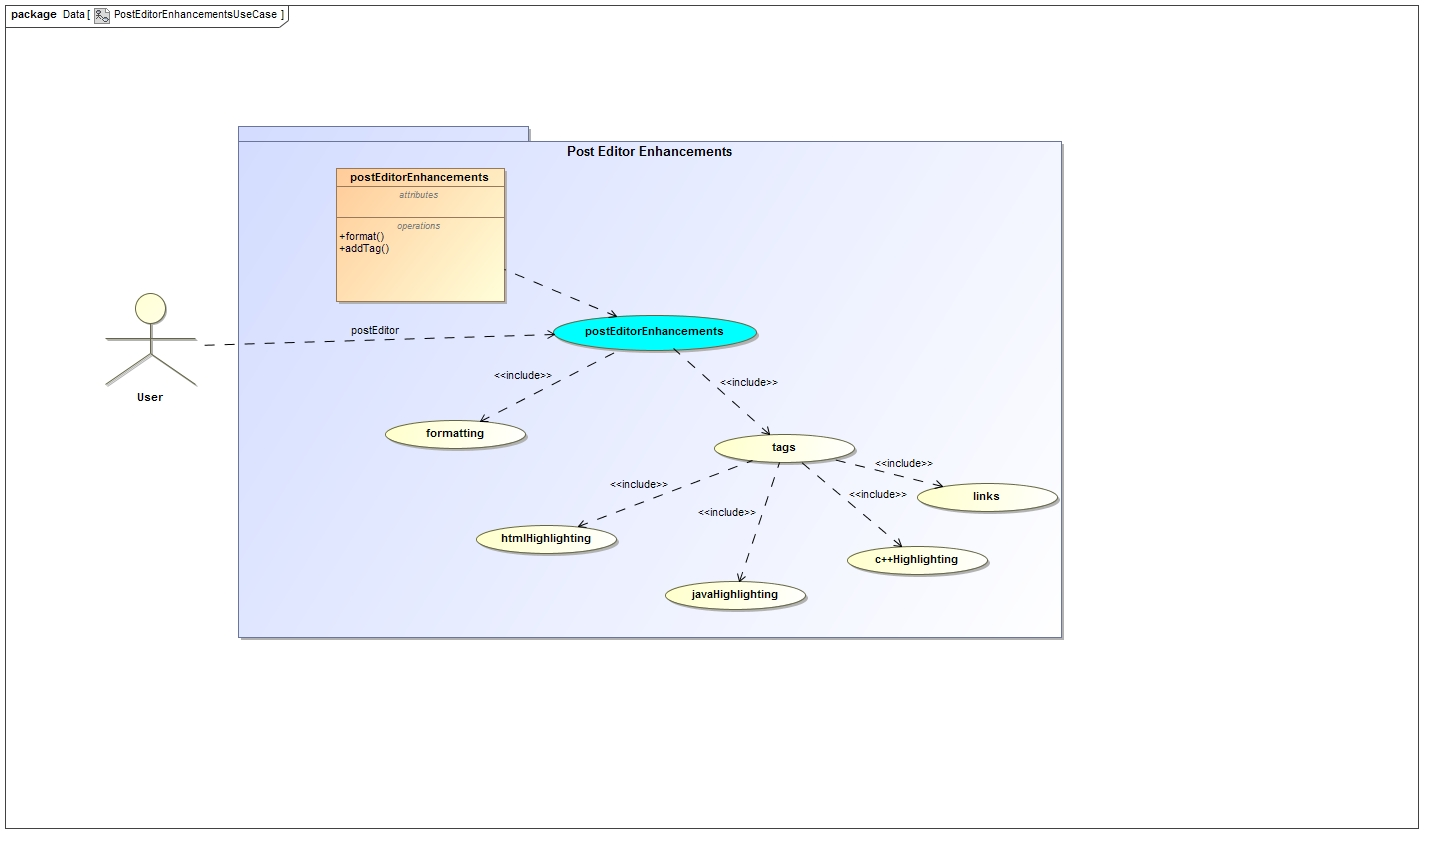
\includegraphics[width=350px]{UseCases/StaffManageContentUseCase.png}
\clearpage %Each point on a new page
   \item  Provide functionality to support semi-automatic creation of thread summaries% Point 6 - Keagan
  \begin{enumerate}
    \item Elaboration – After an allocated user has gone through a thread, selecting the posts that are important enough to be added into the thread summary, the System must process the thread and create the summary using the relevant posts. 
    \item Importance - ***
    \item Dependency level – Relies on the ability to give staff/privileged users the ability to edit threads. It also needs the ranking system as well as a policy governing user levels to be available to it.
    \item Pre-conditions
    \begin{enumerate}
    	\item User must be given the privileges required to view the thread at a higher level and select/unselect posts for inclusion/exclusion in the summary
    	\item Allocated user must submit thread for summarizing to be done by the System
    \end{enumerate}
        \item Post-conditions
    \begin{enumerate}
    	\item User successfully selected the posts that need to be included in the summary and submitted the thread for summarizing
    	\item System processed the thread posts and created one summary of the thread
    \end{enumerate}
    \item Requester – Allocated user
  \end{enumerate}
\begin{figure}[h]
	\centering
	\includegraphics[width=345px]{"Diagrams/Use Case/KT_UC_Point6".jpg}
	\caption{Semi-automatic creation of thread summaries Use Case}
\end{figure}
\begin{figure}[h]
	\centering
	\includegraphics[width=345px]{"Diagrams/Process Specification/KT_AC_Point6".jpg}
	\caption{Semi-automatic creation of thread summaries Activity Diagram}
\end{figure}
\begin{figure}[h]
	\centering
	\includegraphics[width=345px]{"Diagrams/UML/KT_CD_Point6".jpg}
	\caption{Semi-automatic creation of thread summaries Class Diagram}
\end{figure}
\clearpage %Each point on a new page
   \item Create automated template based messages to individual users or specified groups   % Point 7 - Neo
  \begin{enumerate}
    \item Elaboration - This generates a template message about a topic to an individual user or a group.
    \item Importance - ***
    \item Dependency level - This depends on the user input; the system will parse through the user input and build a summary accordingly
    \item Pre-conditions
    \begin{enumerate}
 		\item Condition 1 - Users have to be connected to buzz either logged in or guest account to get automated messages.
    	\item Condition 2 - Group must exist and have at least one member.
    \end{enumerate}
        \item Post-conditions
    \begin{enumerate}
    	\item Condition 1 - Individual user gets a system generated message.
    	\item Condition 2 - Group members get a system generated message.
    \end{enumerate}
    \item Requester - The system.
  \end{enumerate}
	\begin{figure}[h]
    	\centering
    	\includegraphics[width=10cm, height=5cm]{"Diagrams/Use Case/MgsGeneration".png}
    	\caption{Generate template message for user or group.}
    \end{figure}
    
    	\begin{figure}[h]
        	\centering
        	\includegraphics[width=10cm, height=5cm]{"Diagrams/Process Specification/templateBasedMessagesAct".png}
        	\caption{Process specification for generate template message for user or group.}
        \end{figure}
        
        	\begin{figure}[h]
            	\centering
            	\includegraphics[width=10cm, height=5cm]{"Diagrams/UML/templateMessagesCD".png}
            	\caption{Class diagram for generate template message for user or group.}
            \end{figure}
\clearpage %Each point on a new page
   \item Automatically change the status of a user based on the users participation % Point 8 - Matthew
  \begin{enumerate}
    \item Elaboration - The System should be configured in such a way that when a user participates often the user will progress through the levels of the system, Specific number of points required per level.
    \item Importance - ****
    \item Dependency level - Requires the users level to be implemented before a user can participate and increase in level, Users should be able to post on Buzz
    \item Pre-conditions
    \begin{enumerate}
    	\item User is in level x
    	\item User only needs y amount of points to progress
    \end{enumerate}
        \item Post-conditions
    \begin{enumerate}
    	\item User achieved y amount of point
    	\item User is now in level x+1
    \end{enumerate}
    \item Requester - System (Automatically checks each time a user posts)
  \end{enumerate}
\begin{figure}[h]
	\centering
	\includegraphics[width=300px]{"Diagrams/Use Case/PostFreqLevel UseCase".png}
	\caption{Automatically Change users level based on participation Use Case}
\end{figure}
\begin{figure}[h]
	\centering
	\includegraphics[width=300px]{"Diagrams/Process Specification/ProcessSpecUpdateLevel".png}
	\caption{Process Specification for Automatically Update User Level}
\end{figure} 
\begin{figure}[h]
	\centering
	\includegraphics[width=300px]{"Diagrams/UML/UML ChangeUserLevelPosts".png}
	\caption{Automatically Change users level based on participation UML}
\end{figure}
\clearpage %Each point on a new page

   \item Integrate seamlessly with any specified host site. % Point 1 - Syzmon
	\begin{enumerate}
  		\item Elaboration - This process allows owners of the host site to integrate the Buzz space into their site with minimal changes required to their code.
   	 	\item Importance - *****, Critical
   	 	\item Dependency level - The integration of the Buzz Space onto a host site is also important. Host site should not be heavily modified to accommodate the Buzz space, the process must be simple and easy.
   	 	\item Pre-conditions
   		\begin{enumerate}
    		\item Must have host site.
    		\item Must have access to host site.
    	\end{enumerate}
     	\item Post-conditions
    	\begin{enumerate}
  	  		\item Users will be able to interact with one another on Buzz space through the host site.
   	 	\end{enumerate}
   	 	\item Requester - Client
	\end{enumerate}
  	\begin{figure}[h]
  		\centering
  		\includegraphics[width=300px]{"Diagrams/Use Case/Use_Case_Diagram_Integration_with_host_site".png}
  		\caption{Integration of Buzz Space in host site use case diagram}
  	\end{figure}
  	\begin{figure}[h]
  		\centering
  		\includegraphics[width=300px]{"Diagrams/Process Specification/Activity_Diagram_Integration_AD".png}
  		\caption{Integration of Buzz Space in host site activity diagram}
  	\end{figure}
  	\begin{figure}[h]
  		\centering
  		\includegraphics[width=300px]{"Diagrams/UML/Class_Diagram_Site_Integration".png}
  		\caption{Integration of Buzz Space in host site class diagram}
  	\end{figure}
  	\clearpage
  	\newpage
\item Provide functions such as searching and filtering. % Point 10 - Rendani
  \begin{enumerate}
    \item Elaboration - This function will allow users to search for threads by topic, original poster, date etc. and filter posts by the topic such as “assignments”, “practicals”, “tutorials”, “general” etc.
    \item Importance - **
    \item Dependency level - Overall this function does not impact the use of the system and is not critical to the functioning of the system, although it makes navigating through the buzz space somewhat easier.
    \item Pre-conditions
    \begin{enumerate}
    	\item User enters a search query
    	\item User chooses filter condition
    \end{enumerate}
        \item Post-conditions
    \begin{enumerate}
    	\item User is presented with results of search query
    	\item User is presented with filtered threads
    \end{enumerate}
    \item Requester - Client
  \end{enumerate}
  \begin{figure}[h]	
  	\centering
	\includegraphics[width=300px]{"Diagrams/Use Case/SearchingFilteringUseCase".png}
	\caption{Searching and Filtering Use Case}
  \end{figure}
  \begin{figure}[h]
  \centering
	\includegraphics[width=300px]{"Diagrams/Process Specification/SearchActivity".png}
	\caption{Searching and Filtering Activity Diagram}
  \end{figure}
\clearpage %Each point on a new page
   \item  Provide functionality to evaluate posts and vote for posts. % Point 11 - David
  \begin{enumerate}
    \item Elaboration - Users must be able to vote a post up or down. Buzz Space creators must be able to evaluate posts. This will result in more relevant posts getting higher ratings and thus standing out.
    \item Importance - ***
    \item Dependency level - Depends on the post having been created.
    \item Pre-conditions
    \begin{enumerate}
    	\item Post must be created
    \end{enumerate}
        \item Post-conditions
    \begin{enumerate}
    	\item Post is voted up or down.
    	\item Post is evaluated.
    \end{enumerate}
    \item Requester - User
  \end{enumerate}
  	\includegraphics[width=350px]{"Diagrams/Use Case/UseCasePoint11".png}
	  \begin{figure}[h]
  		\centering
  		\includegraphics[width=300px]{"Diagrams/Process Specification/ProcessSpecPoint11".png}
  		\caption{Vote For Posts And Evaluate Posts}
  	\end{figure}
		\begin{figure}[h]
  		\centering
  		\includegraphics[width=300px]{"Diagrams/UML/UML_Point11".png}
  		\caption{Posts UML}
  	\end{figure}
\clearpage %Each point on a new page
   \item Gather statistical information on each user for graphical representation. % Point 12 - Roger
  \begin{enumerate}
    \item Elaboration - System must continuously gather each user’s contribution and participation in the Buzz space to allow the user to view a graphical representation of where they stand or rank up amongst their peers. Provide a game like scoreboard to motivate the users.
    \item Importance - **
    \item Dependency level - Requires the ranking system to be active in order to pull the stats. 
    \item Pre-conditions
    \begin{enumerate}
    	\item User has participated at least x times to gather historical data
    	\item More than y users have contributed to specific Buzz Space
    \end{enumerate}
        \item Post-conditions
    \begin{enumerate}
    	\item User receives the graphical representation of their participation.
    \end{enumerate}
    \item Requester - User
  \end{enumerate}
  \begin{figure}[h]
  	\centering
  	\includegraphics[width=400px]{"Diagrams/Use Case/UserStatisticalinformation UseCase".png}
  	\caption{User Statistical Information Use Case}
  \end{figure}
  \begin{figure}[h]
  	\centering
  	\includegraphics[width=400px]{"Diagrams/Process Specification/UserStatisticalinformation Process Spec".png}
  	\caption{User Statistical Information Process Specification}
  \end{figure}
     \begin{figure}[h]
     	\centering
     	\includegraphics[width=400px]{"Diagrams/UML/UserStatisticalinformation UML".png}
     	\caption{User Statistical Information UML}
     \end{figure}
%Diagram to go here \includegraphics[width=350px]{UseCases/File_Name.png}
\clearpage %Each point on a new page
   \item Enhancement of the post editor % Point 13 - Ivan
  \begin{enumerate}
    \item Elaboration - When a user is posting a reply or creating a new thread there will be options to change formatting or styling of the text as well as embed code within tags to add highlighting and increase readability.
    \item Importance - ***
    \item Dependency level - Relies on a user being allowed to make a post on a thread or create a new thread.
    \item Pre-conditions
    \begin{enumerate}
    	\item User allowed to post reply to thread
    	\item User allowed to create new thread
    \end{enumerate}
        \item Post-conditions
    \begin{enumerate}
    	\item Links posted are allowed
    	\item N/A
    \end{enumerate}
    \item Requester
  \end{enumerate}
%Diagram to go here 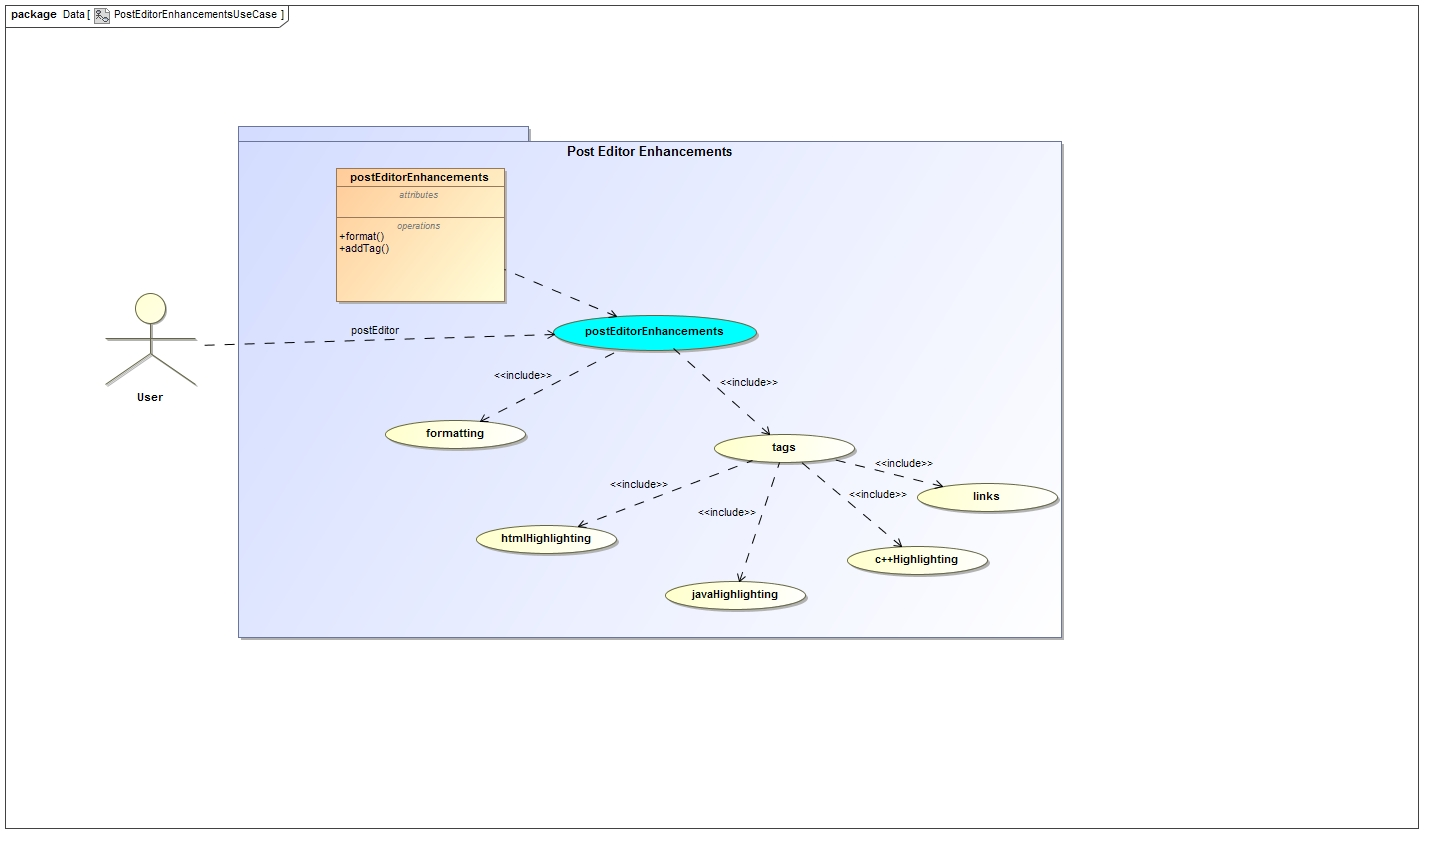
\includegraphics[width=350px]{UseCases/PostEditorEnhancementsUseCase.png}
\clearpage %Each point on a new page
   \item  Provide functions to apply social tagging. % Point 14 - Keagan
  \begin{enumerate}
    \item Elaboration – A user should be able to add a set of tags to his/her own posts as well as to threads/other posts if their user level allows which will be used for more efficient searching of relevant posts. 
    \item Importance - **
    \item Dependency level – Relies on the ranking system being implemented as well as the policy governing user levels so that users with correct privileges can add tags to posts and/or threads.
    \item Pre-conditions
    \begin{enumerate}
    	\item User has correct privileges to add tags to the specific thread/post
    	\item User wants to add tags to thread/post
    \end{enumerate}
        \item Post-conditions
    \begin{enumerate}
    	\item User has entered tag set and tag set has been set for the thread/post.
    \end{enumerate}
    \item Requester – User
  \end{enumerate}
\begin{figure}[h]
	\centering
	\includegraphics[width=345px]{"Diagrams/Use Case/KT_UC_Point14".jpg}
	\caption{Apply Social Tagging Use Case}
\end{figure}
\begin{figure}[h]
	\centering
	\includegraphics[width=345px]{"Diagrams/Process Specification/KT_AC_Point14".jpg}
	\caption{Apply Social Tagging Activity Diagram}
\end{figure}
\begin{figure}[h]
	\centering
	\includegraphics[width=345px]{"Diagrams/UML/KT_CD_Point14".jpg}
	\caption{Apply Social Tagging Class Diagram}
\end{figure}
\clearpage %Each point on a new page
   \item Apply self-organasation based on social tagging and allow the user to view according to the base structure, own structure or public structure % Point 15 - Neo
  \begin{enumerate}
    \item Elaboration - The user is able to use social tags that tell us more about a post thus is also able to search for a thread according to topics that have those social tags and arrange topic threads accordingly via tags. The user is also able to view posts according to the base structure given by the buzz system or specify their own structure by making use of the social tags there is also a general structure for the public who are not registered users. 
    \item Importance - ***
    \item Dependency level - This feature depends on the user selecting tags in which to order the base structure of the posts that they see.
    \item Pre-conditions
    \begin{enumerate}
    	\item Condition - Base structure of posts that is unsorted according to social tags.
    \end{enumerate}
        \item Post-conditions
    \begin{enumerate}
    	\item Condition - Structure that is sorted according to the user's selected organisation of social tags.
    \end{enumerate}
    \item Requester - The user.
  \end{enumerate}
\clearpage %Each point on a new page
    \begin{figure}[h]
    	\centering
    	\includegraphics[width=10cm, height=5cm]{"Diagrams/Use Case/SocialTags".png}
    	\caption{Self-organasation of data via social tags.}
    \end{figure}
    
        \begin{figure}[h]
        	\centering
        	\includegraphics[width=10cm, height=5cm]{"Diagrams/Process Specification/templateBasedMessagesAct".png}
        	\caption{Process specification for self-organasation of data via social tags.}
        \end{figure}
        
            \begin{figure}[h]
            	\centering
            	\includegraphics[width=10cm, height=5cm]{"Diagrams/UML/SocialTagOrganisationCD".png}
            	\caption{Class diagram for self-organasation of data via social tags.}
            \end{figure}
\clearpage %Each point on a new page
   \item Detect if a post is plagiarised  % Point 16 - Matthew
  \begin{enumerate}
    \item Elaboration - The entire post will be checked to see if it has been copied directly from another source, a full post quote will be open searched in a search engine, if any hits are found the post will be marked as possibly plagiarised and send to administrator
    \item Importance - **
    \item Dependency level - User must be able to post to Buzz
    \item Pre-conditions
    \begin{enumerate}
    	\item User posts a post
    \end{enumerate}
        \item Post-conditions
    \begin{enumerate}
    	\item Post is marked as Plagiarised - Added to Buzz(Invisible, Message sent to user and Administrator
    	\item Post is marked as not Plagiarised - Posted to Buzz
    \end{enumerate}
    \item Requester - System, Automatically checks to see if the post is plagiarised.
  \end{enumerate}
\begin{figure}[h]
	\centering
	\includegraphics[width=300px]{"Diagrams/Use Case/Plagiarism UseCase".png}
	\caption{Plagiarism Check Use Case}
\end{figure}
\begin{figure}[h]
	\centering
	\includegraphics[width=300px]{"Diagrams/Process Specification/ProcessSpecPlagiarism".png}
	\caption{Process Specification for Checking Plagiarism API and Internal Checks}
\end{figure}
\begin{figure}[h]
	\centering
	\includegraphics[width=300px]{"Diagrams/UML/UML_Plagiarism".png}
	\caption{Plagiarism Check UML}
\end{figure}
\clearpage %Each point on a new page
   \item Detect violation of netiquette rules. % Point 17 - Syzmon
	\begin{enumerate}
  	\item Elaboration - Many of the users are new to online interaction and often do not know/follow the netiquette rules. This process will check their post against a set of netiquette rules, if the post does not follow these rules the moderator will be notified via e-mail.
   	 	\item Importance - ***, Nice to have
   	 	\item Dependency level - This function is not very important to the system, it is a nice feature to have. The Buzz space can operate without this process.
   	 	\item Pre-conditions
   		\begin{enumerate}
    		\item User must create a post.
    	\end{enumerate}
     	\item Post-conditions
    	\begin{enumerate}
  	  		\item Users post will be created successfully if it follows the netiquette rules.
  	  		\item If the post does not follow one of the netiquette rules, the moderator will be notified about this and post will be flagged.
   	 	\end{enumerate}
   	 	\item Requester - System
  	\end{enumerate}
  	\begin{figure}[h]
  		\centering
  		\includegraphics[width=300px]{"Diagrams/Use Case/Use_Case_Diagram_Netiqutte".png}
  		\caption{Check if post violates netiquette rules use case}
  	\end{figure}
  	\begin{figure}[h]
  		\centering
  		\includegraphics[width=300px]{"Diagrams/Process Specification/Activity_Diagram_Netiquette_check_AD".png}
  		\caption{Check if post violates netiquette rules activity diagram}
  	\end{figure}
  	\begin{figure}[h]
  		\centering
  		\includegraphics[width=300px]{"Diagrams/UML/Class_Diagram_Netiqutte".png}
  		\caption{Check if post violates netiquette rules class diagram}
  	\end{figure}
  \ldots
\end{enumerate}
\end{document}

